\section{Three-tier architecture}

\begin{figure}[H]
    \centering
    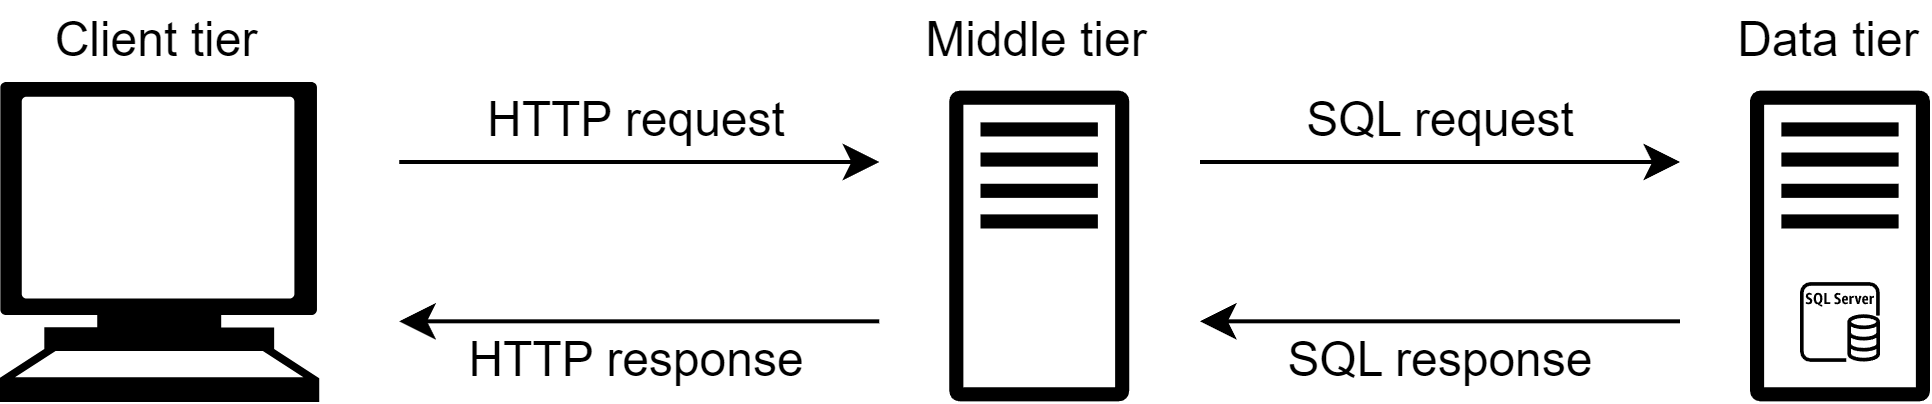
\includegraphics[width=0.5\linewidth]{images/ttph.png}
\end{figure}
The three-tier architecture employs the following hardware components:
\begin{itemize}
    \item Server for data management. 
    \item Client for presentation layout. 
    \item Middle tier to enhance the separation between the client and the server.
\end{itemize}
This architecture has several variants, depending on the software features of the middle tier. 

\paragraph*{Web pure HTML}
In the pure HTML architecture, the client functions as a standard web browser, focusing solely on the presentation layout (thin client). 
The middle tier:
\begin{itemize}
    \item Incorporates a Web server utilizing HTTP.
    \item Hosts the business logic for dynamically generating content from the raw data of the data tier. 
    \item Manages the presentation layout.
\end{itemize}

\paragraph*{Rich internet application}
The rich internet application architecture is the fusion of web and desktop applications (with JavaScript). 
In this scenario, the client is termed fat due to its standard communication protocol (HTTP, Web Socket), language (ECMAScript), and API (DOM, HTML5). 
Noteworthy features of this architecture include:
\begin{itemize}
    \item Novel interface event types, including those specific to touch and mobile apps.
    \item Asynchronous interaction (AJAX).
    \item Client-side persistent data.
    \item Offline application capabilities.
    \item Native multimedia and 3D support.
\end{itemize}